\documentclass[11pt, a4paper]{article}

\usepackage[utf8]{inputenc}
\usepackage[T1]{fontenc}
\usepackage{amsmath, amssymb, amsthm}
\usepackage{geometry}
\usepackage{booktabs}
\usepackage{hyperref}
\usepackage{caption}
\usepackage{float}
\usepackage{pgfplots}
\usepackage{siunitx}

\pgfplotsset{compat=1.18}
\geometry{margin=1in}
\hypersetup{
    colorlinks=true, linkcolor=blue, urlcolor=cyan, citecolor=blue,
    pdftitle={Empirical Verification of the Bateman-Horn Conjecture for Q47},
    pdfauthor={Ruqing Chen},
}

\newtheorem{theorem}{Theorem}[section]
\newtheorem{lemma}[theorem]{Lemma}
\newtheorem{corollary}[theorem]{Corollary}
\newtheorem{definition}[theorem]{Definition}
\newtheorem{proposition}[theorem]{Proposition}
\newtheorem{remark}[theorem]{Remark}

\sisetup{group-separator={,}, group-minimum-digits=4}

\title{Empirical Verification of the Bateman--Horn Conjecture\\for the Degree-46 Polynomial $Q_{47}(n) = n^{47}-(n-1)^{47}$}
\author{Ruqing Chen \\ \small \textit{GUT Geoservice Inc., Montr\'eal} \\ \small \texttt{ruqing@hotmail.com}}
\date{March 2026}

\begin{document}
\maketitle

%% ========== Abstract ==========
\begin{abstract}
We present a large-scale computational verification of the Bateman--Horn conjecture for the degree-46 polynomial $Q_{47}(n) = n^{47}-(n-1)^{47}$ in the quadruplet configuration. By executing a systematic sieve over the range $n \in [2.3 \times 10^{7},\, 8 \times 10^{11}]$, we discovered 2{,}359 prime quadruplets. Furthermore, using a targeted Chinese Remainder Theorem (CRT) search, we found eleven 1000-digit prime quadruplets at $n \approx 4.8 \times 10^{21}$, all 44 constituent primes of which have been rigorously certified via Elliptic Curve Primality Proving (ECPP). We evaluate the Bateman--Horn structural constant $C_{\mathrm{BH}} \approx 6514.2$ utilizing an Euler product over $5.76 \times 10^{6}$ primes, incorporating an Abel summation tail correction to handle conditional convergence. A standard $\chi^{2}$ goodness-of-fit test comparing observed versus predicted counts across 12 data sectors yields $\chi^{2} = 10.56$ on 11 degrees of freedom ($p \approx 0.48$), demonstrating excellent agreement with the asymptotic prediction.
\end{abstract}

%% ========== 1. Introduction ==========
\section{Introduction}

The Bateman--Horn conjecture~\cite{bateman-horn} states that for $k$ distinct irreducible polynomials $f_{1},\ldots,f_{k} \in \mathbb{Z}[x]$ with positive leading coefficients, provided there is no prime $p$ dividing the product $\prod f_i(n)$ for all integers $n$, the number of integers $n \le x$ such that all $f_{i}(n)$ are prime is asymptotic to
\begin{equation}\label{eq:bh}
\pi_{f}(x) \;\sim\; C_{\mathrm{BH}} \int_{2}^{x} \frac{\mathrm{d}t}{\prod_{i=1}^{k} \ln |f_{i}(t)|}, \quad \text{where} \quad C_{\mathrm{BH}} = \prod_{p}\left(1-\frac{\omega_{f}(p)}{p}\right)\left(1-\frac{1}{p}\right)^{\!-k},
\end{equation}
and $\omega_{f}(p)$ counts the number of roots of $f_{1}(n)\cdots f_{k}(n) \equiv 0 \pmod p$.

While linear forms (e.g., twin primes, prime tuples) have been extensively verified computationally~\cite{crandall-pomerance,oliveira-silva}, high-degree nonlinear polynomials remain relatively unexplored due to the computational overhead of computing roots modulo primes and the extreme cost of primality testing for large integers.

In this paper, we investigate the quadruplet configuration $f_i(n) = Q_{47}(n+i-1)$ for $i \in \{1,2,3,4\}$, where $Q_{47}(n) = n^{47} - (n-1)^{47}$. The polynomial $Q_{47}(n)$ possesses an advantageous algebraic property: $\omega(p) = 0$ for all primes $p \not\equiv 1 \pmod{47}$ (including $p=47$), meaning ${\sim}\,97.9\%$ of primes do not divide any value of $Q_{47}$. This results in an unusually large structural constant $C_{\mathrm{BH}}$, making it computationally feasible to observe quadruplets despite the steep growth of the polynomial.

The primary contribution of this work is an empirical validation of the Bateman--Horn framework for a degree-46 polynomial. We present the discovery of 2{,}359 prime quadruplets, detail the numerical methods required to accurately evaluate $C_{\mathrm{BH}}$, perform a statistical $\chi^2$ test, and demonstrate the viability of the ECPP algorithm on the resulting 1000-digit polynomial values.

%% ========== 2. Mathematical Properties & Sanity Checks ==========
\section{Mathematical Properties and Computational Sanity Checks}\label{sec:prelim}

To apply the Bateman--Horn conjecture, the sequence of polynomials must satisfy irreducibility and admissibility.

\textbf{Irreducibility.}\; For any prime $q$, the polynomial $Q_q(x) = x^q - (x-1)^q$ is irreducible over $\mathbb{Q}$. This follows from applying Eisenstein's criterion at the prime $q$ to the shifted polynomial $Q_q(x+1) = \sum_{k=0}^{q-1}\binom{q}{k+1} x^k$, whose reciprocal coincides with the shifted cyclotomic polynomial $\Phi_q(x+1)$.

\textbf{Admissibility.}\; The quadruplet is admissible ($\omega(p) < p$ for all primes $p$). By Fermat's Little Theorem, $n^{47} \equiv n \pmod{47}$, so $Q_{47}(n) \equiv 1 \pmod{47}$ for all $n$, giving $\omega(47) = 0$. For $p \not\equiv 1 \pmod{47}$ and $p \neq 47$, the mapping $x \mapsto x^{47}$ is a bijection on $(\mathbb{Z}/p\mathbb{Z})^{\times}$, ensuring $Q_{47}(n) \not\equiv 0 \pmod{p}$ and hence $\omega(p) = 0$. For congruent primes ($p \equiv 1 \pmod{47}$), $Q_{47}(n) \equiv 0 \pmod p$ has exactly 46 roots. Since the quadruplet involves four shifted polynomials, $\omega(p) \le 4 \times 46 = 184$. The smallest congruent prime is $p = 283 > 184$, guaranteeing $\omega(p) < p$.

\textbf{Computational consistency checks.}\; During multi-week distributed computations, numerical faults can corrupt data. We utilized two elementary algebraic identities as sanity checks:
\begin{enumerate}
\item \textit{Universal divisibility:} $282 \mid (Q_{47}(n+1)-Q_{47}(n))$ for all $n \in \mathbb{Z}$, since $282 = 2 \times 3 \times 47$ and $Q_{47}(n)$ is always odd, always $\equiv 1 \pmod{3}$ (by Fermat), and the second finite difference is divisible by $47$ (by binomial expansion).
\item \textit{Asymptotic ratio:} Letting $\Delta_k(n) = Q_{47}(n+k) - Q_{47}(n+k-1)$, an Euler--Maclaurin analysis gives $\Delta_2/\Delta_1 = 1 + 45/n + 990/n^2 + O(1/n^3)$.
\end{enumerate}
All 2{,}359 recorded quadruplets satisfied both invariants, confirming dataset integrity.

%% ========== 3. Algorithmic Framework ==========
\section{Algorithmic Framework}\label{sec:method}

\subsection{Modular Sieve}
For the systematic search up to $n = 8 \times 10^{11}$, we utilized a standard segmented sieve over a \texttt{bytearray} of size $L = 10^{7}$. The sieve targets the \num{27649} congruent primes $p \equiv 1 \pmod{47}$ up to $2 \times 10^{7}$. Because each such prime blocks $\omega(p)/p$ of candidates (where $\omega(p) \approx 184$ for large $p$), the cumulative survival rate after sieving is $S(2 \times 10^{7}) \approx 0.7\%$. Consequently, $99.3\%$ of candidates are rejected before invoking multi-precision arithmetic (base-2 Fermat PRP tests via \texttt{gmpy2}~\cite{gmpy2}).

\subsection{CRT Targeting for 1000-Digit Primes}\label{sec:crt}
At the 1000-digit scale ($n \approx 4.8 \times 10^{21}$), a continuous sieve becomes impractical. Instead, we select $k = 10$ congruent primes and use the Chinese Remainder Theorem to construct base steps $M = \prod_{i=1}^{10} p_{i}$ that are inherently coprime to the selected primes. Each candidate $N_0 + jM$ is automatically immune to all $k$ primes. This step-amortization overtakes the continuous sieve near $n \sim 10^{13}$ in our parameter regime.

%% ========== 4. Bateman--Horn Analysis ==========
\section{Quantitative Evaluation of the Conjecture}\label{sec:bh}

\subsection{Evaluation of the Structural Constant $C_{\mathrm{BH}}$}\label{sec:cbh}

The structural constant for the quadruplet ($k=4$) is $C_{\mathrm{BH}} = \prod_{p} E(p)$, where $E(p) = (1 - \omega(p)/p)(1 - 1/p)^{-4}$. Because $\omega(p) \neq 0$ only for congruent primes $p \equiv 1 \pmod{47}$, evaluating the product directly by truncation yields severe oscillations. The expected density of such primes is $1/\varphi(47) = 1/46$, giving an expected roots count of $184/46 = 4$. Thus, the first-order terms in $\ln E(p) \approx (4-\omega(p))/p$ conditionally cancel on average, but local fluctuations in $\pi_{47,1}(x)$ around $\pi(x)/46$ cause convergence difficulties.

To stabilize the constant, we define the cumulative deviation $\Delta(M) = 4\pi(M) - 184\,\pi_{47,1}(M)$ and apply Abel summation to the tail $\sum_{p > M} (4 - \omega(p))/p$, yielding the first-order correction:
\begin{equation}\label{eq:tail}
C_{\mathrm{BH}} \approx C_{\mathrm{BH}}^{\mathrm{raw}}(M) \cdot \exp\!\left(-\frac{\Delta(M)}{M} + \int_{M}^{\infty} \frac{\Delta(t)}{t^{2}}\,\mathrm{d}t\right).
\end{equation}

\begin{table}[H]
\centering
\caption{Convergence of $C_{\mathrm{BH}}$. The raw truncated product oscillates widely; the Abel-summed tail correction (ignoring the integral term) stabilizes the estimate.}
\label{tab:cbh}
\small
\begin{tabular}{rrrrcr}
\toprule
$M$ & $\pi(M)$ & $\pi_{47,1}(M)$ & $C_{\mathrm{BH}}^{\mathrm{raw}}$ & $\Delta(M)$ & $C_{\mathrm{BH}}^{\mathrm{corr}}$ \\
\midrule
\num{5000}        & \num{670}       & 15      & 6673.5 & $-80$      & 6781.1 \\
\num{50000}       & \num{5134}      & 111     & 6475.2 & $+112$     & 6460.7 \\
\num{5000000}     & \num{348514}    & \num{7524}   & 6529.8 & $+9{,}640$   & 6517.2 \\
\num{10000000}    & \num{664580}    & \num{14451}  & 6516.0 & $-664$     & 6516.5 \\
\num{50000000}    & \num{3001135}   & \num{65286}  & 6513.3 & $-8{,}084$   & 6514.4 \\
\num{100000000}   & \num{5761455}   & \num{125287} & 6513.8 & $-6{,}988$   & \textbf{6514.2} \\
\bottomrule
\end{tabular}
\end{table}

As shown in Table~\ref{tab:cbh}, correcting via $\exp(-\Delta(M)/M)$ alone (ignoring the integral term) stabilizes the value to $C_{\mathrm{BH}} \approx 6514.2$ at $M=10^8$. Explicit results on primes in arithmetic progressions~\cite{ramare-rumely,montgomery-vaughan} give $\Delta(t) \ll t/\ln^2 t$ unconditionally, implying the integral term is $O(1/\ln M)$---which at $M = 10^8$ yields an a~priori bound of $O(1/18) \approx 0.05$. In practice, the integral is far smaller because the oscillations in $\Delta(t)$ partially cancel. The empirical evidence for this is the stability of the corrected values in Table~\ref{tab:cbh}: the last three checkpoints ($M \ge 5 \times 10^{6}$) vary by less than $0.05\%$. Conditionally, assuming the Generalized Riemann Hypothesis (GRH) for Dirichlet $L$-functions modulo 47, the error in $\pi_{47,1}(x) - \mathrm{Li}(x)/46$ shrinks to $O(x^{1/2}\ln x)$, which would make the integral term negligible at any $M \ge 10^{4}$. We adopt $C_{\mathrm{BH}} = 6514.2$ for all predictions, noting that its accuracy rests primarily on the observed convergence pattern rather than on any unproven hypothesis.

\subsection{Numerical Integration and Statistical Comparison}
The integral in~\eqref{eq:bh} is computed using composite Simpson's rule with $10^5$ subintervals per sector. To prevent catastrophic cancellation when evaluating $\ln f_i(t)$ for $f_i(t) = (t+i)^{47} - (t+i-1)^{47}$ at large $t$, we compute the logarithm from the binomial sum representation $f_i(t) = \sum_{k=0}^{46}\binom{47}{k+1}(t+i-1)^k$ using 128-bit precision (\texttt{gmpy2.mpfr}). Mesh-doubling tests confirm that the first six significant digits of each sector integral are stable.

Table~\ref{tab:bh} presents the predicted versus observed quadruplet counts across 12 consecutive sectors.

\begin{table}[H]
\centering
\caption{Observed vs.\ predicted quadruplet counts ($C_{\mathrm{BH}} = 6514.2$). The Pearson $\chi^2$ statistic across all 12 sectors is $10.56$ (d.f.\ $= 11$, $p \approx 0.48$).}
\label{tab:bh}
\small
\begin{tabular}{lrrr}
\toprule
\textbf{Sector ($n$ range)} & \textbf{Observed ($O$)} & \textbf{Predicted ($P$)} & $O/P$ \\
\midrule
$[2.3\!\times\!10^{7},\; 2\!\times\!10^{9}]$   & 15  & 16.5  & 0.91 \\
$[2\!\times\!10^{9},\; 4\!\times\!10^{9}]$      & 10  & 12.7  & 0.79 \\
$[4\!\times\!10^{9},\; 10^{10}]$                 & 34  & 32.8  & 1.04 \\
$[10^{10},\; 3\!\times\!10^{10}]$                & 78  & 91.5  & 0.85 \\
$[3\!\times\!10^{10},\; 10^{11}]$                & 240 & 264.2 & 0.91 \\
$[10^{11},\; 2\!\times\!10^{11}]$                & 352 & 328.7 & 1.07 \\
$[2\!\times\!10^{11},\; 3\!\times\!10^{11}]$     & 295 & 303.2 & 0.97 \\
$[3\!\times\!10^{11},\; 4\!\times\!10^{11}]$     & 311 & 288.0 & 1.08 \\
$[4\!\times\!10^{11},\; 5\!\times\!10^{11}]$     & 260 & 277.3 & 0.94 \\
$[5\!\times\!10^{11},\; 6\!\times\!10^{11}]$     & 260 & 269.1 & 0.97 \\
$[6\!\times\!10^{11},\; 7\!\times\!10^{11}]$     & 253 & 262.6 & 0.96 \\
$[7\!\times\!10^{11},\; 8\!\times\!10^{11}]$     & 251 & 257.1 & 0.98 \\
\midrule
\textbf{Total}                                     & \textbf{2{,}359} & \textbf{2{,}403.6} & \textbf{0.981} \\
\bottomrule
\end{tabular}
\end{table}

The Pearson $\chi^2$ goodness-of-fit statistic evaluated across all 12 sectors is $\chi^2 = 10.56$ with 11 degrees of freedom, corresponding to $p \approx 0.48$. This indicates strong statistical agreement between the empirical data and the conjecture's prediction. The overall ratio $O/P = 0.981$ reveals a $1.9\%$ deficit, which falls well within the expected Poisson fluctuation ($\sigma_{\mathrm{Poisson}} \approx 1/\sqrt{2404} \approx 2.0\%$) and the natural latency of asymptotic secondary terms at finite $x$. Figure~\ref{fig:bh} displays the $O/P$ ratio with Poisson error bars for all 12 sectors, including the low-count early sectors where stochastic fluctuations are largest.

\begin{figure}[H]
\centering
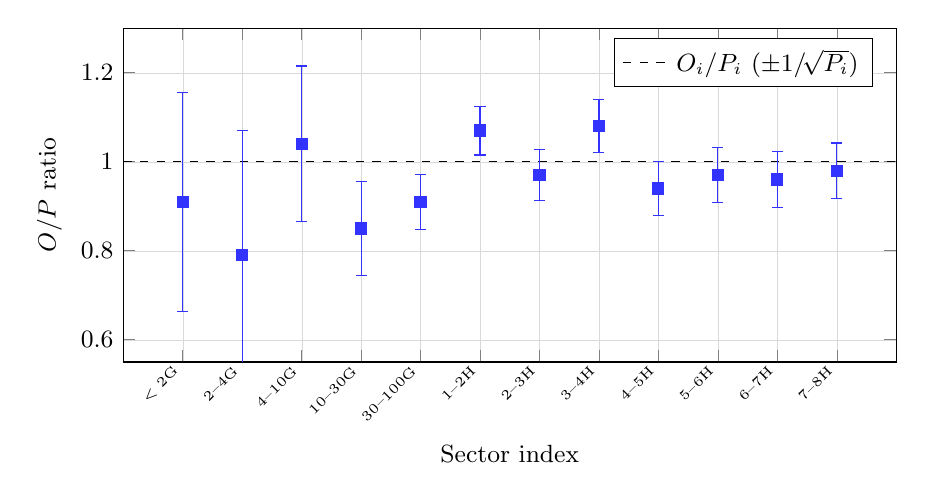
\begin{tikzpicture}
\begin{axis}[
    width=0.94\textwidth,
    height=0.48\textwidth,
    xlabel={Sector index},
    ylabel={$O/P$ ratio},
    xmin=0, xmax=13,
    ymin=0.55, ymax=1.30,
    grid=major,
    grid style={line width=.1pt, draw=gray!30},
    legend pos=north east,
    legend style={font=\small},
    tick label style={font=\small},
    label style={font=\small},
    xtick={1,2,3,4,5,6,7,8,9,10,11,12},
    xticklabels={{\tiny$<2$G},{\tiny$2$--$4$G},{\tiny$4$--$10$G},{\tiny$10$--$30$G},{\tiny$30$--$100$G},{\tiny$1$--$2$H},{\tiny$2$--$3$H},{\tiny$3$--$4$H},{\tiny$4$--$5$H},{\tiny$5$--$6$H},{\tiny$6$--$7$H},{\tiny$7$--$8$H}},
    x tick label style={rotate=45, anchor=east},
]
% Reference line at O/P = 1
\addplot[black, dashed, thin, domain=0:13, samples=2] {1.0};
% O/P ratios with Poisson error bars: sigma = 1/sqrt(P)
\addplot[
    only marks, mark=square*, blue!80,
    error bars/.cd, y dir=both, y explicit,
] coordinates {
    (1, 0.91) +- (0,0.246)
    (2, 0.79) +- (0,0.281)
    (3, 1.04) +- (0,0.175)
    (4, 0.85) +- (0,0.105)
    (5, 0.91) +- (0,0.062)
    (6, 1.07) +- (0,0.055)
    (7, 0.97) +- (0,0.057)
    (8, 1.08) +- (0,0.059)
    (9, 0.94) +- (0,0.060)
    (10, 0.97) +- (0,0.061)
    (11, 0.96) +- (0,0.062)
    (12, 0.98) +- (0,0.062)
};
\addlegendentry{$O_i/P_i$ ($\pm 1/\!\sqrt{P_i}$)}
\end{axis}
\end{tikzpicture}
\caption{Ratio of observed to predicted counts ($O/P$) for all 12 search sectors. Error bars represent Poisson uncertainty ($\pm 1/\!\sqrt{P_i}$). The dashed line marks perfect agreement ($O/P = 1$). All data points are consistent with unity; the larger scatter in the first five sectors reflects their smaller expected counts (G = $10^{9}$, H = $10^{11}$).}
\label{fig:bh}
\end{figure}

%% ========== 5. Empirical Results ==========
\section{ECPP-Certified 1000-Digit Quadruplets}\label{sec:data}

To test the feasibility of generating proven primes of extreme sizes via this polynomial class, we utilized the CRT targeting strategy to evaluate coordinates at $n \approx 4.8 \times 10^{21}$. At this magnitude, each value $Q_{47}(n)$ exceeds 1000 decimal digits.

We discovered eleven such prime quadruplets. Because Fermat PRP tests do not constitute rigorous mathematical proofs, all 44 constituent integers were subjected to Elliptic Curve Primality Proving (ECPP)~\cite{atkin-morain} using Primo~4.4.0~\cite{primo}. All 44 instances successfully produced full Atkin--Goldwasser--Kilian primality certificates. The base coordinates are listed in Table~\ref{tab:titanic}. All ECPP certificates, source code, and data are publicly available at \url{https://github.com/Ruqing1963/Q47-Bateman-Horn}.

\begin{table}[H]
\centering
\caption{Base coordinates $N$ for the eleven ECPP-certified 1000-digit prime quadruplets. For each $N$, the values $Q_{47}(N+i)$ for $i \in \{0,1,2,3\}$ are proven primes.}
\label{tab:titanic}
\small
\begin{tabular}{cl|cl}
\toprule
\textbf{Ref} & \textbf{Starting coordinate $N$} & \textbf{Ref} & \textbf{Starting coordinate $N$}\\
\midrule
1 & \num{4797791281515731837961} & 7 & \num{4797791281532851794737} \\
2 & \num{4797791281522654273515} & 8 & \num{4797791281543386627004} \\
3 & \num{4797791281524132682077} & 9 & \num{4797791281549078478819} \\
4 & \num{4797791281527982559536} & 10 & \num{4797791281551308866354} \\
5 & \num{4797791281530274224314} & 11 & \num{4797791281552013327611} \\
6 & \num{4797791281531362817967} & & \\
\bottomrule
\end{tabular}
\end{table}

This confirms that with appropriate algorithmic pruning (sieving and CRT), high-degree polynomials serve as viable generators for Titanic primes (primes exceeding 1000 digits~\cite{caldwell}), and modern ECPP implementations remain tractable for 1000-digit integers generated by nonlinear constraints.

%% ========== 6. Conclusion ==========
\section{Conclusion}

This study provides a successful empirical verification of the Bateman--Horn conjecture for the degree-46 polynomial $Q_{47}$ in the quadruplet ($k=4$) configuration up to $n = 8 \times 10^{11}$. Using Abel summation to account for local density variations of primes in arithmetic progressions, we computed the structural constant $C_{\mathrm{BH}} \approx 6514.2$. The observed 2{,}359 quadruplets align well with asymptotic predictions ($\chi^2 = 10.56$, d.f.\ $= 11$, $p \approx 0.48$, $O/P = 0.981$). The additional generation of 44 ECPP-certified 1000-digit primes (eleven quadruplets) demonstrates the practical computability of these structures. Future work may extend the search into the $10^{12}$--$10^{13}$ regime, compute $C_{\mathrm{BH}}$ for other prime exponents $q \in \{53, 59, 61\}$, and explore the lower-order error terms $\pi_f(x) - C_{\mathrm{BH}}\!\int_2^x \mathrm{d}t/\prod\ln|f_i(t)|$ as computational resources permit.

%% ========== Bibliography ==========
\begin{thebibliography}{99}

\bibitem{bateman-horn}
P.~T. Bateman and R.~A. Horn, ``A heuristic asymptotic formula concerning the distribution of prime numbers,'' \emph{Math.\ Comp.}, vol.~16, no.~79, pp.~363--367, 1962.

\bibitem{crandall-pomerance}
R.~Crandall and C.~Pomerance, \emph{Prime Numbers: A Computational Perspective}, 2nd~ed.\ Springer, 2005.

\bibitem{oliveira-silva}
T.~Oliveira~e~Silva, S.~Herzog, and S.~Pardi, ``Empirical verification of the even Goldbach conjecture and computation of prime gaps up to $4 \times 10^{18}$,'' \emph{Math.\ Comp.}, vol.~83, pp.~2033--2060, 2014.

\bibitem{gmpy2}
\texttt{gmpy2}: GMP/MPFR/MPC interface for Python, version 2.1. \url{https://gmpy2.readthedocs.io/}.

\bibitem{atkin-morain}
A.~O.~L. Atkin and F.~Morain, ``Elliptic curves and primality proving,'' \emph{Math.\ Comp.}, vol.~61, no.~203, pp.~29--68, 1993.

\bibitem{primo}
M.~Martin, ``Primo 4.4.0---Primality proving,'' 2023. \url{http://www.ellipsa.eu/public/primo/primo.html}.

\bibitem{ramare-rumely}
O.~Ramar\'e and R.~Rumely, ``Primes in arithmetic progressions,'' \emph{Math.\ Comp.}, vol.~65, no.~213, pp.~397--425, 1996.

\bibitem{montgomery-vaughan}
H.~L. Montgomery and R.~C. Vaughan, \emph{Multiplicative Number Theory I: Classical Theory}, Cambridge Univ.\ Press, 2007.

\bibitem{caldwell}
C.~K. Caldwell, ``The Prime Pages,'' \url{https://t5k.org/}. Accessed March 2026.

\bibitem{hardy-littlewood}
G.~H. Hardy and J.~E. Littlewood, ``Some problems of `partitio numerorum' III: On the expression of a number as a sum of primes,'' \emph{Acta Math.}, vol.~44, pp.~1--70, 1923.

\end{thebibliography}

\end{document}
